\documentclass[a4paper]{jlreq}
\usepackage[haranoaji]{luatexja-preset}

\usepackage{amsmath, amssymb}
\usepackage{bm}
\usepackage{siunitx}
\usepackage{listings}

\usepackage{graphicx}
\usepackage{svg}
\usepackage{wrapfig}

\begin{document}
  \title{document}
  \author{Actat}
  \date{}
  \maketitle

  \section{ロボット製作の動機}

  このロボットの製作に取り組むのは,歩行ロボット製作を経験するためである.
  最終的には二足歩行ロボットの製作を目指しているが,6自由度の脚の設計は難易度が高いと判断し,
  今回は3自由度の脚を4つ備えた四足歩行ロボットを製作することにした.

  このロボットの製作では以下の内容を経験することを期待している.
  \begin{itemize}
    \item 自宅でのロボット製作
    \item サーボモータを用いた機構の設計
    \item 最低限の電気回路の取扱い
    \item ROSを用いたプログラミング
    \item 歩行ロボットの制御
  \end{itemize}

  \section{機械設計・製作}

  設計・製作したロボットを図\ref{fig:robot}に示す.
  脚は前後左右に鏡像になっている同一の機構とした.
  サーボモータは研究室で使用しているモータと合わせて近藤科学株式会社のB3M-SC-1170-Aを用いた.
  CIT Brainsが公開しているB3Mモータを用いた二足歩行ロボットを参考に,関節間の距離は\SI{100}{mm}にした.

  胴体中央下部に株式会社アールティのUSB出力9軸IMUセンサモジュールを搭載した.
  センサの位置をロボットのベースリンクと一致させて計算を簡単にする意図がある.
  胴体上部前方に取り付けられた板にサーボモータとPCの間の通信のための基板を固定した.

  \begin{figure}[htb]
    \centering
    \input{robot.pdf_tex}
    \caption{
      設計・製作したロボット
    }
    \label{fig:robot}
  \end{figure}

  \section{電装}

  ロボット全体で12個のモータが使われている.
  モータとパソコンはRS485USB/シリアル変換アダプターを介して通信する.
  直列に接続できるモータの数は限られているので
  XHコネクター用ハブ typeAによって各脚ごとの系統に分けて接続した.
  配線の様子を図\ref{fig:wiring}に示す.

  XHコネクター用ハブには5つのコネクタがあり,すべて並列に接続される.
  このハブはロボット前方に横向きに取り付けられており,
  中央のコネクタをRS485USB/シリアル変換アダプターに接続し,
  左右のコネクタをそれぞれ脚のモータと接続した.
  脚の3つのモータはHip flexion/extension, Hip ab/adduction, kneeの順に接続された.
  Hipのモータは機械的な接続とは逆の順序である.

  \begin{figure}[htb]
    \centering
    \input{wiring.pdf_tex}
    \caption{
      配線の様子
    }
    \label{fig:wiring}
  \end{figure}

  サーボモータは配線に先立ってIDの書き込みを行った.
  書き込んだIDは表\ref{table:servo_id}に示すとおりである.

  \begin{table}[htb]
    \caption{IDと関節の対応}
    \label{table:servo_id}
    \centering
    \begin{tabular}{rcc}
      \hline
      id & 脚 & 関節 \\
      \hline
      0 & 左前 & Hip ab/adduction \\
      1 & 左前 & Hip flexion/extension \\
      2 & 左前 & knee \\
      3 & 右前 & Hip ab/adduction \\
      4 & 右前 & Hip flexion/extension \\
      5 & 右前 & knee \\
      6 & 左後 & Hip ab/adduction \\
      7 & 左後 & Hip flexion/extension \\
      8 & 左後 & knee \\
      9 & 右後 & Hip ab/adduction \\
      10 & 右後 & Hip flexion/extension \\
      11 & 右後 & knee \\
      \hline
    \end{tabular}
  \end{table}

  \section{Packageの作成}

  別のディレクトリで
  \texttt{\$ ros2 pkg create --build-type ament\_cmake --node-name quadruped\_takahashi quadruped\_takahashi}
  を実行してpackage.xml, CMakeLists.txt, quadruped\_takahashi.cppを作成した.
  その後,作成したファイルをこのリポジトリ内へ移動した.

  \section{モータとの通信}

  モータとの通信にはActat/kondo\_b3m\_ros2を用いる.
  motor\_classブランチ\footnote{このプロジェクトでうまく動作することを確認したらmasterにする予定である.}に合わせて
  launchファイルを用意し,通信ができることを確認する.
  以下にlaunchファイルのうち,kondo\_b3m\_ros2のノードの設定に関する部分を抜粋する.
  軸の方向を反転しているのは,後述する座標系に合わせるためである.

  \begin{lstlisting}[basicstyle=\ttfamily, language=Python]
    kondo_b3m_ros2_node = Node(
      package='kondo_b3m_ros2',
      executable='kondo_b3m',
      remappings=[('b3m_joint_state', 'joint_states')],
      parameters=[{'motor_list': [
        "{'id': 0, 'name': 'lf0', 'direction': False}",
        "{'id': 1, 'name': 'lf1', 'direction': False}",
        "{'id': 2, 'name': 'lf2', 'direction': False}",
        "{'id': 3, 'name': 'rf0', 'direction': False}",
        "{'id': 4, 'name': 'rf1'}",
        "{'id': 5, 'name': 'rf2'}",
        "{'id': 6, 'name': 'lh0'}",
        "{'id': 7, 'name': 'lh1', 'direction': False}",
        "{'id': 8, 'name': 'lh2', 'direction': False}",
        "{'id': 9, 'name': 'rh0'}",
        "{'id': 10, 'name': 'rh1'}",
        "{'id': 11, 'name': 'rh2'}"
      ]}],
    )
  \end{lstlisting}

  あるウインドウで\texttt{\$ ros2 launch quadruped\_takahashi launch.py}を実行して起動し,
  別のウインドウで\texttt{\$ ros2 topic echo /joint\_states}することで各関節の角度・角速度が出力されていることを確認した.

  \section{URDFファイルの作成}

  URDFファイルの作成にあたってロボットの関節に関する座標系を設定する.
  初めに左前脚を考える(図\ref{fig:lfleg_coords}).
  2つのHipの関節は軸が交わるように作られており,この交点を脚の付け根とする.
  脚の付け根を原点としてロボットの前方に$x$軸,左方向に$y$軸,鉛直上方向に$z$軸をとった座標系を$\Sigma_\mathrm{lf0}$とする.
  $\Sigma_\mathrm{lf0}$の$x$軸はHip ab/adductionの関節軸と一致しており,
  この軸周りに$\theta_\mathrm{lf0}$回転した座標系を$\Sigma_\mathrm{lf1}$とする.
  $\theta_\mathrm{lf0}$は$x$軸の方向を正とする.
  $\Sigma_\mathrm{lf1}$の$y$軸はHip flextion/extensionの関節軸と一致しており,
  この軸周りに$\Sigma_\mathrm{lf1}$回転した座標系を$\Sigma_\mathrm{lf2}$とする.
  $\Sigma_\mathrm{lf1}$は$y$軸の方向を正とする.
  この座標系$\Sigma_\mathrm{lf2}$は腿のリンクと対応しており,腿は$-z$の方向にのびている.
  膝関節は$\Sigma_\mathrm{lf2}$において$[0, 0, -0.1]\,\si{m}$の位置に存在する.
  この位置を原点とし,$y$軸周りに$\theta_\mathrm{lf2}$回転した座標系を$\Sigma_\mathrm{lf3}$とする.
  この座標系は脛のリンクと対応しており,$[0, 0, -0.1]\,\si{m}$の位置が足の球の中心になる.

  \begin{figure*}[htb]
    \centering
    \input{fig_lfleg_coords.pdf_tex}
    \caption{
      左前脚の座標系の設定.
      脚は3つの関節軸を持っておりそれぞれが独立に回転する.
      脚を垂直に伸ばした状態で2つの尻関節の交点と足の球面の中心を結ぶ線分上に各座標系の原点を設定する.
      それぞれの関節の回転角を$\theta_\mathrm{lf0}, \theta_\mathrm{lf1}, \theta_\mathrm{lf2}$とする.
    }
    \label{fig:lfleg_coords}
  \end{figure*}

  他の脚にも同様に3つの関節角と4つの座標系を定義する.
  すべて座標軸は直立したときに,$x$軸が前方,$y$軸は左方を向くように設定する.
  関節角の向きは$x, y$軸の正方向によって定める.

  ロボットの中心となるbase\_linkの位置は,4つのhip jointの中心に定める.
  座標系の向きは$x$軸が前方,$y$軸は左方,$z$軸が鉛直上方である.

  URDFファイルを作成して,CMakeLists.txtに追記した.
  rvizのconfigファイルも同様にCMakeLists.txtに追記した.
  launch.pyを編集し,rvizを起動して/joint\_statesの関節角をモデルの表示に反映させる.
  base\_linkを固定して表示させることができた(図\ref{fig:urdf_rviz_screen}).

  \begin{figure*}[htb]
    \centering
    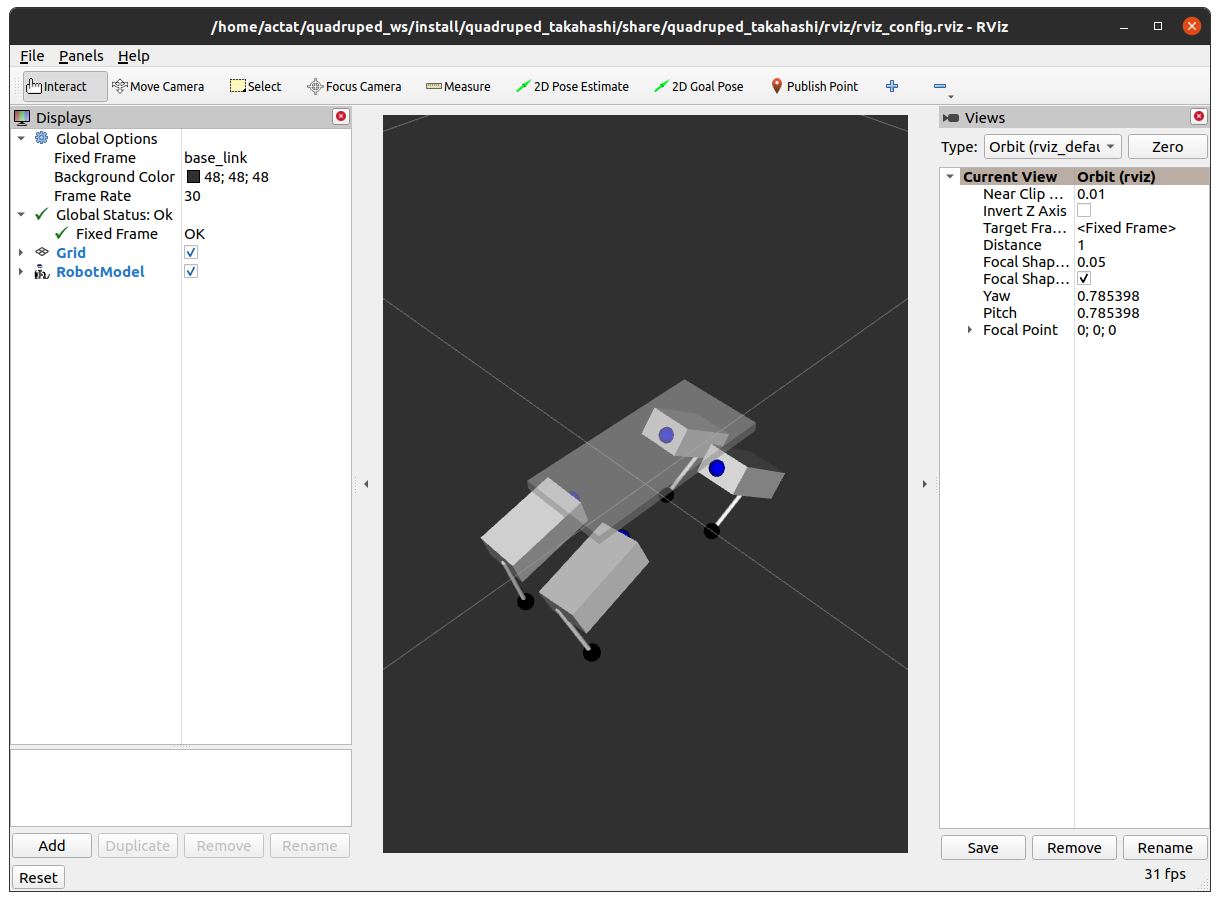
\includegraphics[width=15cm]{urdf_rviz_screen.png}
    \caption{URDFファイルを読み込んで表示するrvizの画面}
    \label{fig:urdf_rviz_screen}
  \end{figure*}

  \section{IMUのデータを読み取る}

  胴体中央下部に株式会社アールティのUSB出力9軸IMUセンサモジュールが搭載されている.
  rt-net/rt\_usb\_9axisimu\_driverによってrosのtopic(/imu/data\_rawと/imu/mag)にデータをパブリッシュする.
  パブリッシュされたデータはCCNYRoboticsLab/imu\_toolsのimu\_complementary\_filterで姿勢の情報にする.
  使用するパッケージをpackage.xmlに追記し,launchファイルにノードを起動する記述を追加した.

  \texttt{odom}から\texttt{base\_link}への\texttt{tf}をパブリッシュする
  \texttt{quadruped\_takahashi\_odometry}というノードを作る.
  \texttt{/imu/data}をサブスクライブし,更新が入ったらコールバックで足の情報を参照して\texttt{tf}に情報を出す.
  ひとまず$xy$平面内での位置はゼロに固定し,高さは最も低い位置にある足が接地しているものとする.

\end{document}
